\documentclass[../physical_computing.tex]{subfiles}

\begin{document}

\chapter{Lab Exercise 4 - Joining and Sharing Components}
\label{sec:appendix_5}

\section{Motivation and Overview}
\label{sec:motivation}

In Appendices \ref{sec:appendix_2}, \ref{sec:appendix_3} and \ref{sec:appendix_4} we used as examples a binary counter, a de-bounced push-button, and writing to a seven segment LED display. In this chapter, we shall use these three projects as components of a device that counts how many times you have pressed a push-button and displays the count in hexadecimal on the display. We shall do this in several different ways, and as an aside we shall learn how to use, and then how to set up, a shared repository for code using the sharing infrastructure of \git.

\section{Using a git repository}
\label{sec:usegit}

A public git repository containing VHDL code for a debounced button, a sixteen bit counter, and a driver for the four digit display on the BASYS3 board can be found at \url{https://github.com/eddaw1/phyip}. Go to this repository. You will find yourself in the main directory and see before you several folders, including three that I will want you to use in this lab. These are 
\texttt{bgate}, which contains IP for a debounced button, \texttt{sixteencount}, IP for a sixteen bit binary counter triggered by 
an active-high logic pulse, and \texttt{sevenseg}, a code for driving the seven segment display. Descend into each subdirectory in turn. Note that the \texttt{..} link in the subdirectory takes you back up a level to the main \texttt{phyip} directory. Within each subdirectory, you will see two further subdirectories, called \texttt{src} and \texttt{gui}. These contain, respectively, the VHDL source code and a file that allows Vivado to generate a graphical user interface (GUI) widget corresponding to the IP device. We will first use the \texttt{port map} mechanism to write code connecting the pieces of IP into a project. 

\subsection{Connecting up IP using \texttt{port map}}
\label{sec:portmap}

The \texttt{port map} mechanism allows you to connect input and output ports of the IP elements together to form a larger program, rather like calling functions within the body of a program in a high level language. To connect together the elements from my IP catalog, you'll need to start a new Vivado project in the usual way. Specify the usual constraint file, uncomment the lines associated with the clock, the 7 segment LED display (decimal point, anodes, and segments), and the central button on the 5-button pad. Now within the project, you are going to create four new VHDL files, and copy the VHDL code from my IP repository corresponding to the debounced button, the counter, and the display driver into three of these three VHDL files. The fourth file is for the port map statements to link them together. You can do this by creating empty VHDL files, then copying and pasting the code form my repository into the empty files. Call the files \texttt{sevenseg.vhd}, \texttt{counter.vhd}, \texttt{debouncedbutton.vhd} and \texttt{toplevel.vhd}. You can add all three files at once using the \texttt{Add Sources} link in the top left of the Vivado GUI. There is no need to use this link three times separately for the three files, though it does no harm if you do. You do not need to specify any particular inputs or outputs to these files.

Now go in to \texttt{counter.vhd}, and completely empty it out. On the git repository web site. Descend into the \texttt{sixteencount\/src} subdirectory, and click on \texttt{sixteencounter.vhd}. This will then show you a source listing of the VHDL for the IP. Click on the \texttt{raw} button in the top right corner of the code pane, and you will see an ascii dump of the code. Empty the \texttt{counter.vhd} file in your Vivado project. Back in the git repository, highlight the code, crtl-c to copy it, and in VHDL ctrl-v to paste it into the \texttt{counter.vhd} file in your Vivado project. 

Repeat this exercise, pasting the contents of the git repository file \\
\texttt{bgate/src/32bit\_counter.vhd}, which contains the debounced button, into the Vivado project \texttt{debouncedbutton.vhd} file, and the contents of the git repository file 
\texttt{sevenseg/directlight.vhd} into the git repository file \texttt{sevenseg.vhd}. Three out of the four VHDL files in your Vivado project should now be populated. Save them all. As you do this, check for the appearance of syntax errors in the files. It is quite easy to make a mistake and forget to delete the last line or the first line that the newly created VHDL file came with when you paste in the contents of the git repository, for example. 

Next you need to create the port map file that connects everything together. Go in to \texttt{toplevel.vhd}. Using the notes from seminar 6, yesterday, create three port maps that connect together the three pieces of IP with internal signals to interconnect between the three IP blocks and ports for inputs and outputs. The only input ports should be clk and the button, and the output ports should be the anodes, segments, and decimal point, of the 4 digit LED display.

\section{Your first VIVADO GUI}
\label{sec:firstvivadogui}

The \texttt{port map} mechanism is, as I said in the lecture, rather cumbersome. Though it gets the job done and sometimes not having to mess about with a graphical user interface can be faster, and more efficient, there is no way of really visualising the functionality of the code you are writing. The Vivado GUI mechanism, where you represent each piece of IP with a graphical widget and join them with wires, is a natural way to overcome these problems. We can exploit this mechanism to build up the same project as we just went through with \texttt{port map}, graphically.

The instructions for doing this are again in the notes for seminar 7 from yesterday. Starting at slide 20, open a terminal and use \texttt{git clone} to copy my entire git repository onto your laptop. Then follow the instructions on Slides 21-30 to build up a connected block diagram connected to the same ports as in the port map version. Finally create an overarching master vhdl file and build and run your counter. Specific instructions that mirror the contents of seminar 7 are given in Section \ref{sec:createblockdesign}.

\subsection{Drawing a block design}
\label{sec:createblockdesign}

Once the main VIVADO window is open, look in the top left corner for 'Create Block Design'. The default name of design\_1 is fine. Hit OK.
We are going to want to add our own IP blocks to this design, so we need to tell Vivado where to look for them. They should all be in the my\_ip local git repository copy. Right-click on the open design window, and select `IP settings'. In the left-hand menu of the window that appears, flip open the option labelled IP by clicking on the arrow, and select 'Repository'. A small box should appear, labelled IP repositories, which is initially empty. Click on '+' and navigate to my\_ip. When you select this directory, you should see this appear in the `Add repository' window, and there should be at least 3 IP blocks, one for each of your mini projects. Click OK and OK again to close the IP settings window.

You next need to add one copy of each of the debouncer, the sixteencounter and the seven segment display. Click on the '+' button to add IP. An enormous list will appear, containing many interesting possibilities - a very large stack of pre-configured IP arrives with the Vivado package. Fortunately there is also a search engine that should permit you to find your three pieces of IP using the names they had when you exported them as IP - probably these will be the same names as those of the VHDL source files they were created from. As you add these IPs to the project you 
will see their gui representations appear in the window, and things should look very much as they do in Figure \ref{fig:guione}.

\begin{figure}[htbp]
    \centering
    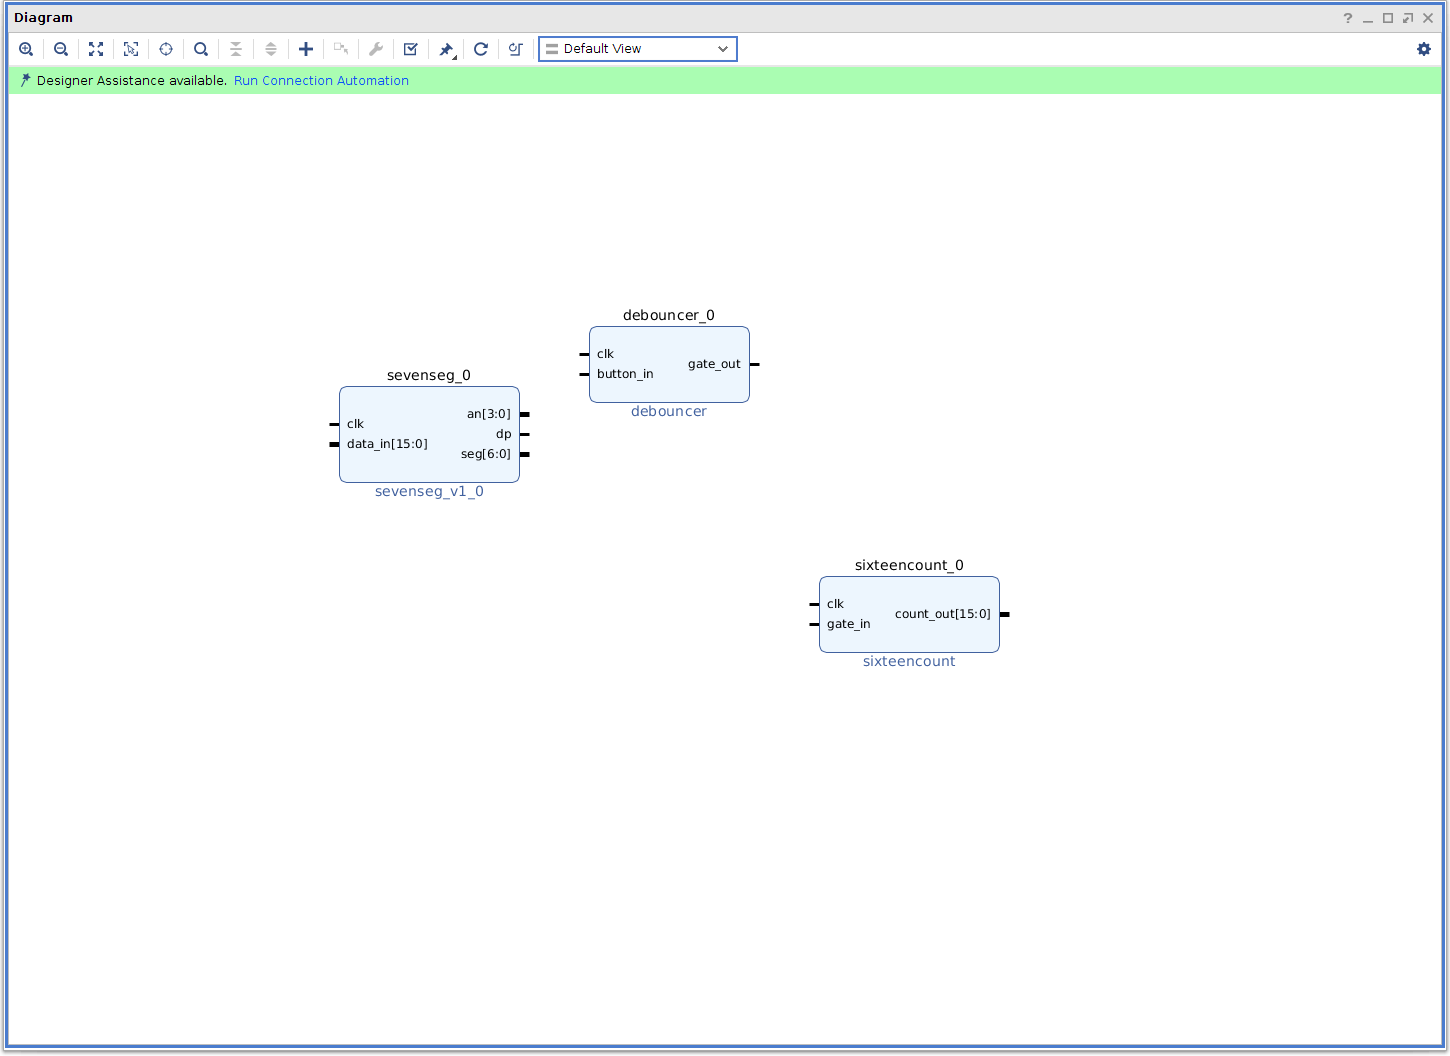
\includegraphics[width=0.8\textwidth]{appendix_5/figures/guione.png}
    \caption{The gui window before wiring but after the IP elements of our design are added.}
    \label{fig:guione}
\end{figure}

You should play with the GUI window a bit. If you left click and drag diagonally in the window, it either magnifies or zooms out on the gui window. If you find yourself lost, you can click on the third icon at the top from the left, which is 'zoom to fit' and will fit whatever graphics you have imported into your view in the window. You should rearrange them so that the debounced button is on the left, the counter is in the middle and the display driver is on the right. Then wire the internal connections by dragging wires between ports until it looks roughly as it does in Figure \ref{fig:guitwo}.

\begin{figure}[htbp]
    \centering
    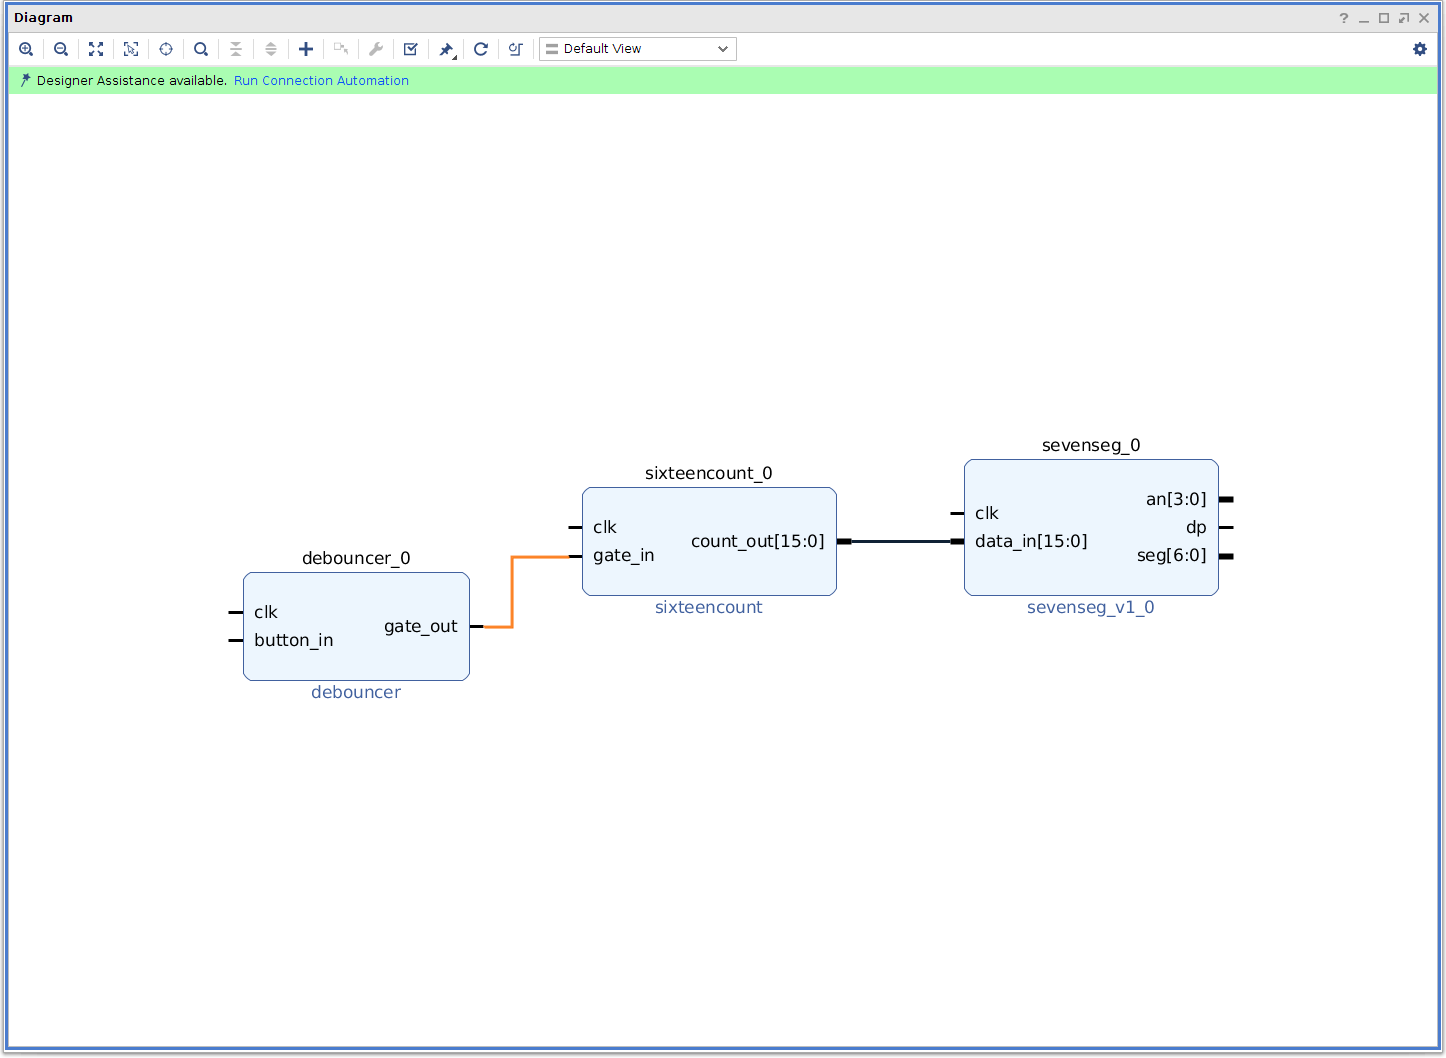
\includegraphics[width=0.8\textwidth]{appendix_5/figures/guitwo.png}
    \caption{The gui window after internal wires but before external wires.}
    \label{fig:guitwo}
\end{figure}

We have now connected all the internal wires, those that don't join to any ports - pins on the actual chip. All three of our widgets require a clock input. If you hover over the clk input to the debouncer, and right click then select 'Make external', it will create a wire to an external input. Repeat this for button\_in, and on the seven segment display for both output ports (mine has an additional ouptut for the decimal point, so I've connected that too, but you needn't worry about this. Now you can also join wires from the clock inputs to the other two widgets to the same input port for the clock as for the debouncer, and it should create neat wires connecting all three clock inputs to the same input port. Things will look very much like they do in Figure \ref{fig:guithree}.

\begin{figure}[htbp]
    \centering
    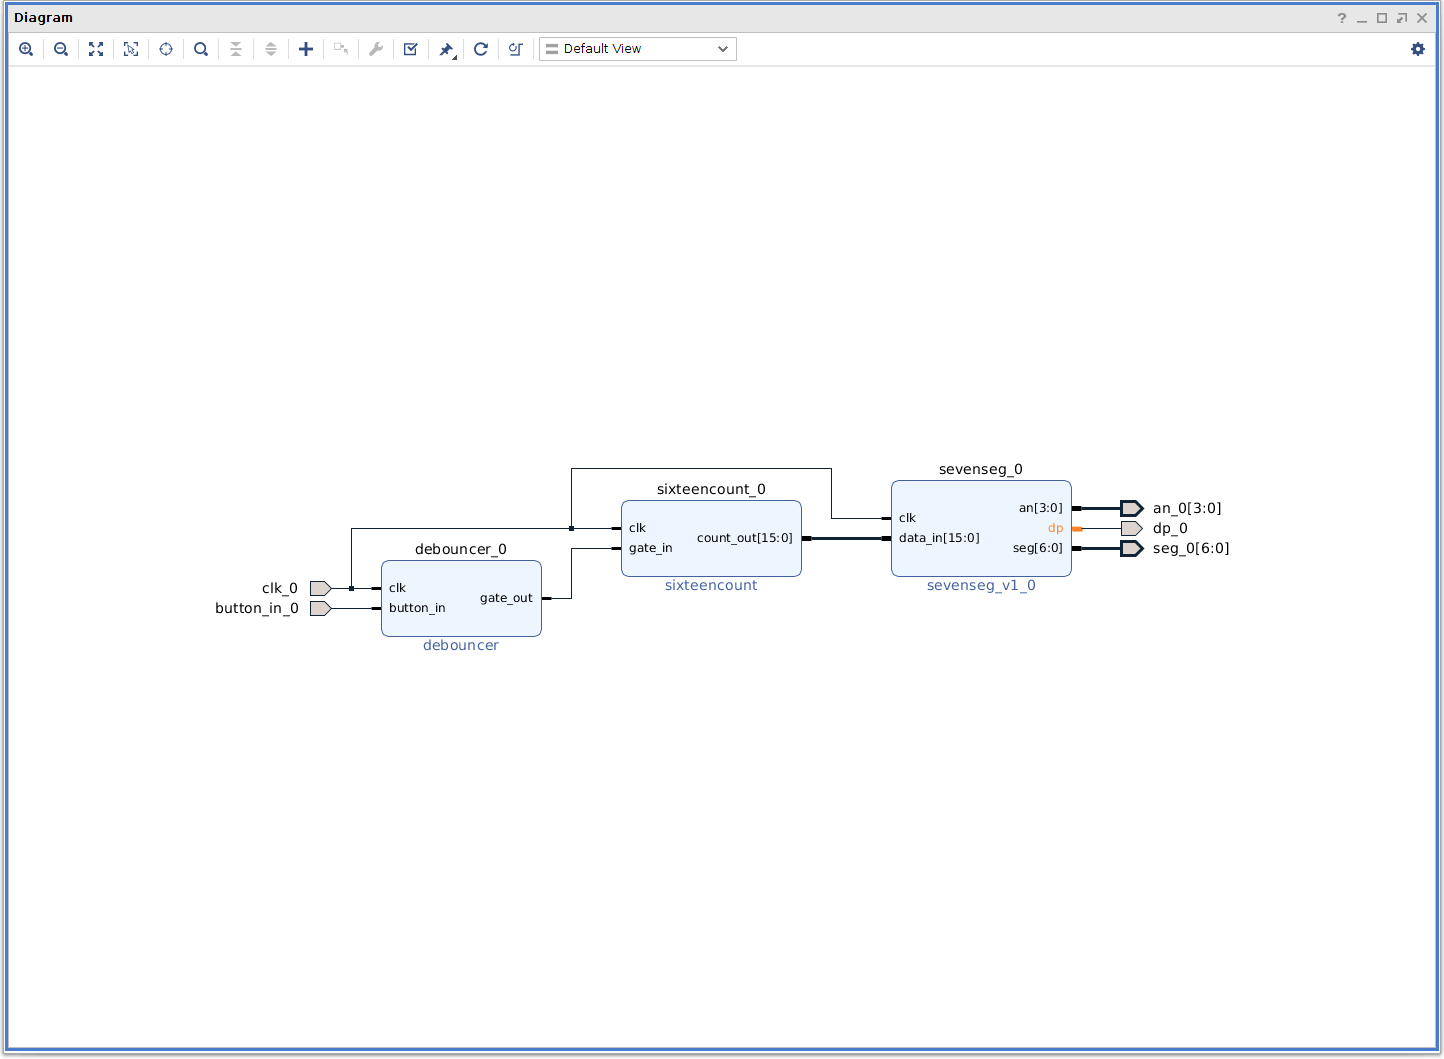
\includegraphics[width=0.8\textwidth]{appendix_5/figures/guithree.png}
    \caption{The gui window with all wires in place.}
    \label{fig:guithree}
\end{figure}

One slightly annoying habit of this gui is adding \_0 after the name of each port that is made into an external input or output. These either have to be added by hand in the constraint file, or they have to be edited in the gui. The latter is less fussy. Simply click on each port in turn, and a window at the lower left of the GUI pane should appear called `External Port Properties'. The names I suggest are clk, btnC, an, and seg. These will then match the corresponding names in the constraints file. Finally, edit the constraints file and make sure each port that you are going to use is uncommented. Save the constraint file. Save the block design in the file menu. And, make sure the constraint file is saved.

One remaining step before we build. The gui is in fact just a graphical user interface to VHDL, and therefore we need an overarching VHDL file into which this gui fits. To create one, go to the 'Sources' tab in the top left of the main Vivado window, and highlight design\_1, your block design. Right click on it and select `Create HDL wrapper'. 

You are now ready to build the project. Click `Run Synthesis' as usual. This will take a little longer than usual because each of the IP sub-blocks needs to get built before the project as a whole is put together. This is where having multiple cores on your laptop is useful - one core can be deployed for each IP build in parallel, which speeds things up noticeably. If you are curious about how things are progressing, go to the 'Design runs' tab in the slim pane at the bottom, and open the sub-area called 'Out-of-Context module runs', and at the bottom of that hierachy you should be able to see things building.

Once the synthesis has finished, you should be able to proceed as usual with Run Implementation and Generate Bitstream. Hopefully when you write the bitstream, you will be able to use the central pushbutton to increment the digital display counter. Though this was a simple project, you can see that the graphical method gives you a much more visual picture of what is going on in the code. The power of this method is fully exploited when building large systems on the chip that include processors, memory, input terminals, and shared memory with your own modules.

If you get done with this exercise, and successfully build your debounced button driven counter, you might want to try
one of the following exercises.

\begin{itemize}
    \item Create a git repository using the instructions in Section \ref{sec:gitrepo} below.
    \item Use the built in IP called DSP48E1 in Vivado to make a simple adder for two numbers that explicitly uses the DSP slice.
\end{itemize}

\section{Starting your own git repository}
\label{sec:gitrepo}

A git repository is the current standard for sharing and team development of code. You can, and we will learn how to, store your created IP in a git repository, then retrieve it and use the copy to deploy into a new git project. Others can (with your permission) also download your developed IP, and many users can also collaborate on the same code, even at the same time using a mechanism called branching. Here we will only go as far a simple example, a repository containing just the IP for your 32 bit binary to hex display converter. So, the first job is to create your own account on github, if you don't have one. Visit the URL \url{https://github.com}, and follow the instructions to open a new account. in the left hand vertical menu bar that appears, to the right of the word 'Repositories', there should be a button labelled 'New', which you click, and are then prompted to provide a name for your repository. I suggest you call it phyip. Once you have created it, you can return to github home by clicking on the cat silouette in the top left corner. Then you can click on phyip under Repositories to enter the new repository. It is currently empty. 

The next step is to ensure that you can check your code into the repository. To do this we will create an encryption key pair between your laptop and your git repository. On the laptop type in the following:

\begin{minted}{shell}
ssh-keygen -t rsa -b 4096 -C "physics"
\end{minted}

Accept the default location for the file, which is in your home directory under a hidden subdirectory called .ssh (all directories and files whose name begins with a dot are normally hidden, but you can see them using ls -a). Also when prompted for a passphrase, leave it blank, and again when asked to re-enter it. Now if you invoke

\begin{minted}{shell}
cd /home/physics/.ssh
ls
\end{minted}

you should be able to see two new files in there, \texttt{id\_rsa.pub} and
\texttt{id\_rsa}. These are your public and private keys. The basic rules of key encryption is that the private keys never leave your machine, but the public keys can be shared with anyone. 

In the web page for github, inside your new phyip project, at the top there are a horizontally justified set of tabs, including a settings tab which you should click. Close to the bottom of the left justified vertical list of options, you should see `deploy keys'. Click this option, and then click AddDeployKey. This should bring up an empty box. In the terminal window you have open in your .ssh directory, type more id\_rsa.pub. Several lines of seemingly random alphanumeric characters starting in ssh-rsa and ending in physics should appear. If you left-click-drag over the whole thing, then middle-click in the AddDeployKey box in your github deploy keys window, then the whole string should get copied over. Next give it the title `physics' and click `Add Key'. This gives your computer remote access to the git repository from the terminal command line. Your new repository is now ready to drop your code onto.

Next, cd into the \texttt{/home/physics/my\_ip} directory. A subdirectory for your display IP should already be there. The next job is to create a generic readme file called README.md. To do this type nano README.md. This should open a blank text editor window in your terminal. Type in a sentence of explanation of what the repository is for. Now do ctrl-O to write the file, and ctrl-X to exit the editor. 

You are now ready to make the local directory into a git repository and push to your github account. You should still be in the \texttt{my\_ip} directory, and this is going to be the top directory of your git repository. From there, do the following

\begin{minted}{shell}
git init
# the < and > symbols should not be included, they just prompt
# you to replace the carets and their contents with something
# personal to you.
git config --global user.email "<your email>"
git config --global user.name "<your name>"
git add --a
git commit -a
\end{minted}

When you do git commit, you'll be put into a nano editor window, and there you type some description of what you just did to the code - in this case
something like repository creation is appropriate. Use ctrl-O (accept default filename) and ctrl-X to exit. Now to create a shortcut to your github repository. In the command below, put your github username where I 
have inserted the carets.

\begin{minted}{shell}
git remote add origin git@github.com:<username>/phyip.git
git branch -M main
git push -u origin main
\end{minted}

Now if you refresh your browser window in the github site, you should be able to see entries for the README.md file and the displayhex IP directory. Congratulations! Your first developed HDL code is now on git. If you want, you can make it public and others can download and use it. We'll have a go at cloning a git repository back to your machine and making use of it next.

\section{Use of github to store VHDL source for use with \texttt{ port map}}
\label{sec:githubportmap}

For the purpose of storing VHDL source for use with the \texttt{port map} mechanism, it suffices to store only the VHDL source that corresponds to the device you have created. For example, you may wish to store devices for the pushbutton debouncer and the LED display. It will be important to organise things so that our git repository does not get cluttered. Let us therefore agree on an organisational framework for our repository. Within the phyip project, let us create a subdirectory called portmapsources. Within this subdirectory we will create a further subdirectory for each piece of VHDL that is intended to be used with the \texttt{port map} mechanism. So, within the \texttt{my\_ip} subdirectory on your laptop (so you will need to \texttt{cd my\_ip} in a terminal window, make new subdirectories for each piece of VHDL code you want to store.

\begin{minted}{shell}
cd my_ip
mkdir debouncebutton
mkdir leddisplay
git add debouncebutton
git add leddisplay
\end{minted}

The \texttt{git add} commands don't do anything to the remote repository - nothing happens remotely until you invoke \texttt{git push}. Next \texttt{cd} into each of the subdirectories in turn, and in that subdirectory create a \texttt{README.md} file using
\texttt{nano README.md}. This file should contain what the VHDL code does, your name and email. I would advise against putting a date of creation because git is much better at keeping track of that than you are likely to be. Dates written in to files become defunct almost immediately and it is impossible to keep track of all of them.

Now it is time to go and find the VHDL code that you used in the Exercise of Section \ref{sec:portmap}. The actual VHDL file you created is in the directory containing the Vivado project where you tested your portmap under 
\begin{minted}{vhdl}
/<project name>.srcs/sources_1/imports/<username>/<filename> 
\end{minted}
Use cp to copy this file into the correct subdirectory of your git repository, the same directory where you created the \texttt{README.md} file that tells you where it is. Now \texttt{cd} back to \texttt{my\_ip} and in that directory invoke:
\begin{minted}{shell}
# adds all the new files to the git project
git add -A
# commits the current version of the files - you'll
# need to do this each time you modify them.
git commit
\end{minted}
Once again you'll be taken into the nano editor - write some text explaining what you just added to the repository, then do ctrl-O (and accept the default file name) to write the file and ctrl-X to exit the editor. Nothing you have done so far will affect the repository on github. However, now we are ready to push the new version to the github repository. 
\begin{minted}{shell}
git push -u origin main
\end{minted}
If all has gone well, your VHDL code should now be safely backed up to the repository. 

If this seems like an awfully convoluted way of backing up a file, then you are right - it is! But, the advantages of this method of keeping a backup quickly becomes apparent when you are developing software in a team, or are interested in publishing what you have written.

Git supports an otherwise problematic side of software development called version control. Suppose there were 100 developers working on a massive \texttt{VHDL} project, and all of them were modifying some subset of the files all the time. How would you keep track of these things? Git supports branching, where you can create a `branch' of the repository, check out the code, make changes and check back in without actually merging your changes in a way that affects other developers. Whenever the repository managers agree that everyones changes are going to be combined together, then the repository manager can carefully merge everyones changes back onto the master repository. And, when everything works again (usually after some problems with incompatibilies - you can't escape that one!), the master repository can be `tagged', so that if someone breaks the master branch, it is possible to rewind to the last time it worked and thereby fix it. 

Another advantage is that github supports a secure web interface, which we have been using already to view what is in our repository. In fact, if you go back to your github repository view on the web and use the browser refresh, you should be able to see the new folder structure and its file contents on the web interface. You can also edit the files there, but bear in mind that there is no way to test your edits by building the VHDL code into bitstream files and programming the board remotely, so any edits done on the web interface to the repository should be done with extreme care. One neat thing about the github web interface is that github `knows' the syntax for a wide range of languages, including VHDL! So if you use the web interface to view your source code you'll find the comments, commands and keywords are colour coded for easier code browsing. 

Finally, Git supports controlled public release of your software. You can let the entire internet look at your source, but nobody that you don't want to be altering your code is allowed write access. So, if you think your debounced pushbutton works particularly well, you can launch it onto the web and who knows? Perhaps it will be in a cellphone somewhere before you know it!

\section{Packaging for the VIVADO GUI}
\label{sec:vivadogui}

The \texttt{port map} paradigm is perfectly functional and flexible enough to support quite sophisticated large project integration from modular small pieces. The main limitation is that it doesn't lend itself to quick debugging. It is hard to see for any remotely complicated module, based on the port map syntax, exactly how things are wired together, and it is easy to make mistakes, as you may already have found. Also, you have to know exactly how to connect everything, down to the individual wire. This isn't so bad when you have a 3 port device such as the debouncer, but what happens when your device is a microprocessor? You shouldn't have to figure out exactly hwo to wire everything! It would be nice if modules could come with some built in native intelligence so they in some sense `know' how they should be wired up. For example, we shall soon see that we can grab a module that is a fully functional microprocessor called microblaze. This processor will want to be connected to memory. The memory is also available - we don't have to write it (thank goodness). We also, it turns out, don't have to know exactly how to connect the memory to the processor. This can all be coped with in vivado using a hand graphical user interface that they supply with the package. We will now learn how to deploy our IP so that it can be used with this package. It is surprisingly easy. After that, we'll learn how to deploy our graphics-ready widget to github so that others can use it.

Reopen the VIVADO project where you previously created and tested the \texttt{ port map} to the 3 port debounced button core. The VHDL for this core itself is in a subdirectory of that project, called
\begin{minted}{shell}
/<project name>.srcs/sources_1/imports/<username>/<filename> 
\end{minted}
It is this VHDL file that we want to package up as a GUI widget that can be used in the vivado graphical developer. In the VIVADO project (you should previously have verified that the button debouncer works - you can just as easily carry out this exercise using the 4 digit LED display driver, so long as you have a working submodule that was successfully accessed using the \texttt{port map} protocol.

In the open VHDL project, first ensure that the hardware manager is closed. In the `tools' menu at the top, select 'Create and Package new IP...'. In the sub-window that appears, have a read of the verbage, then click Next. The default in the next window is to package the whole project. But we don't want to do this, because the whole project interfaces the debouncer to a specific button on a specific board. What we want to export is just the VHDL that debounces a generic button, potentially on a generic board, even perhaps using an FPGA made by a different manufacturer, or perhaps this VHDL code will be used to design an application specific integrated circuit (ASIC) - a much more specialised (and expensive) proposition! So, instead we check the box that says
'Package a specified directory', and again click Next. We then navigate to the directory containing the VHDL code for the debouncer. Mine is called \texttt{debouncer.vhd} and it is in the directory above. So click in the `...' box, and navigate to the directory containing that file. There is no need to check the 'package as a library core' button, though we may come back to what this button is for later. Click `Next'.

You next want to create a directory where the packaged IP will eventually be written. We want this to be in the local copy of our git repository. So, in the shell, 
\begin{minted}{vhdl}
cd /home/physics/my_ip
mkdir -p guiwidgets/debouncedbutton
\end{minted}

Leave the contents of the `Project location' box at the default; this is where Vivado creates the temporary project it uses to build the GUI.
Click `Next' again. Then, click `Finish'.

Vivado will then launch a completely separate project to package up the debouncer into a GUI widget. It might take a minute or two and the computer fans may come in. It seems to have quite a lot to do - who knows what. Anyway, what you see next should look like Figure \ref{fig:makeguiscreen1}.

\begin{figure}[htbp]
    \centering
    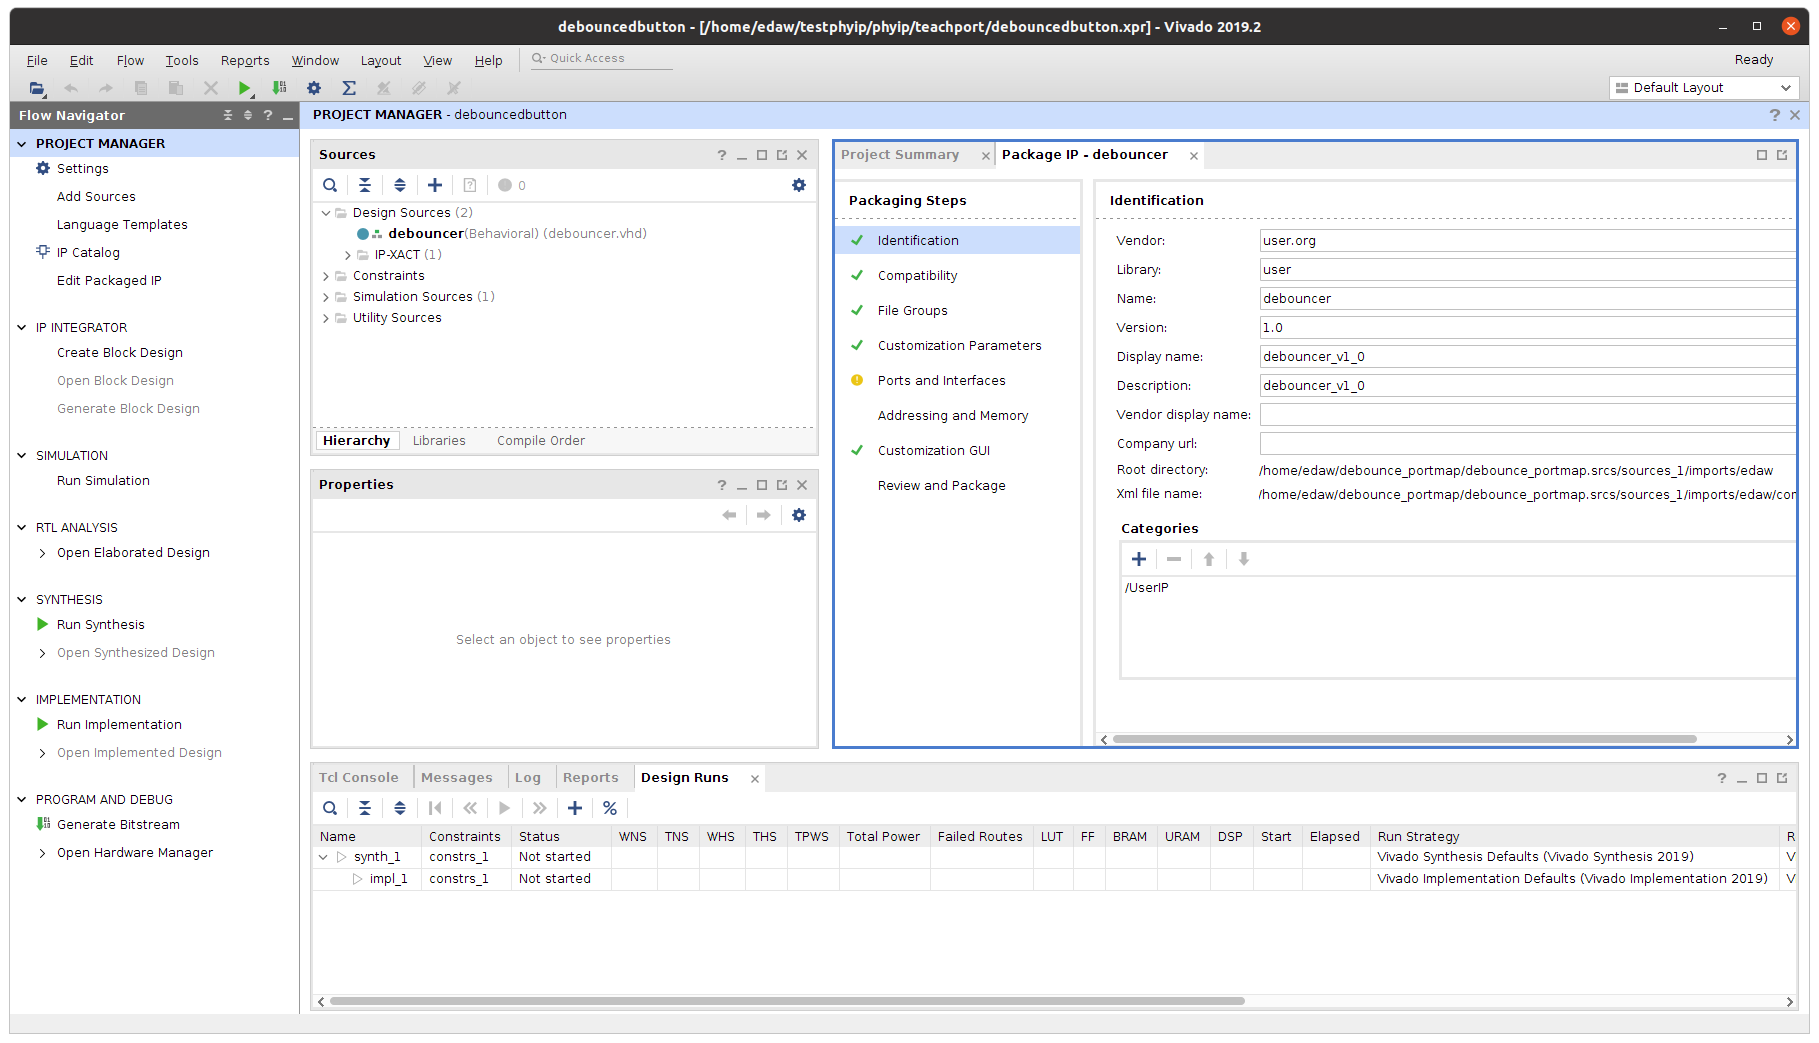
\includegraphics[width=0.8\textwidth]{appendix_5/figures/makeguiscreen1.png}
    \caption{The sub-project containing the source for the widget export. Widgets are called IP by Vivado - they are thinking that you are going to become a developer and sell these things...maybe you will!}
    \label{fig:makeguiscreen1}
\end{figure}

The thing to look at here is the main pane, containing the `Package IP - debouncer' tab. This contains some fields that you might care about if you were going to sell your widget to someone. Here we will leave most of them as defaults. The one thing we will change is the Display name, because these \_v1\_0 labels will appear in all our GUIs if we don't. Alter debouncer\_v1\_0 to just plain debouncer.

Next, click on the menu item to the left of this tab called `customisation GUI'. this is what your tool will look like when you incorporate it into a graphical project. The GUI widget for my debouncer is shown in Figure \ref{fig:debouncergui}. Inputs are on the left, outputs are on the right. There is lots of flexibility built in to this gui creation tool, since it is probably also used to create the IP for processors, memory, sophisticated bus devices, etc. But for us it is sufficient to create something very simple. 

\begin{figure}[htbp]
    \centering
    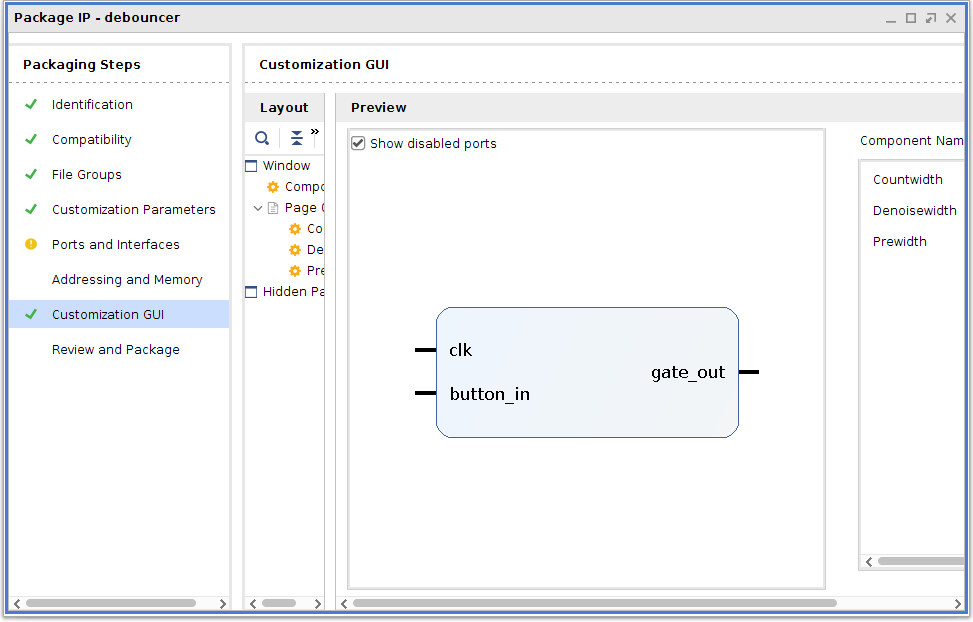
\includegraphics[width=0.5\textwidth]{appendix_5/figures/justmywidget.png}
    \caption{This is the graphical representation of the debouncer widget. Inputs are on the left, outputs are on the right.}
    \label{fig:debouncergui}
\end{figure}

If all seems well, then click on the 'Review and Package IP' item in the vertical bar to the left of the GUI sketch, and select package IP. It should say that it has finished successfully, and ask you if you want to close the project - select Yes. You can now also close the project containing the port map 'container' that you used to test port mapping.

Now to put your newly created IP in the git repository. In a terminal window, go into the sources directory where the VHDL code you just created is located.
\begin{minted}
{shell}
cd .../<project name>.srcs/sources_1/imports/<username>
ls
\end{minted}

In addition to \texttt{debouncer.vhd} you should now be able to see a file called \texttt{component.xml}
and a directory called \texttt{xgui}. This whole structure needs to be copied into your local copy of the GIT repository 

\begin{minted}
{shell} 
cp -R * /home/physics/my_ip/guiwidgets/debouncedbutton/.
\end{minted}

Next move to the local copy of the git repository, add the new files, commit, and push to the git repository

\begin{minted}
{shell}
cd /home/physics/my_ip
git add -A
git commit
# enter what you are changing in nano, 
# then ctro-O, return, ctrl-X
git push -u origin main
\end{minted}

You should now refresh your browser view of the git repository and go and take a look at the files you have uploaded under the new directory path to guiwidgets that should have appeared. One nice thing about VHDL is that when it exports IP cores like this, only a very minimal set of files is dumped to the IP core directory. These files include the VHDL source, a description of functionality in the ascii text format XML, and a script in a language called Tcl that is used by Vivado in incorporating your IP core into other projects. You don't have to worry about exactly what these files are, but you might wish to take a look at them in the web git interface, just for interest.

\end{document}